\documentclass[tikz,border=5pt]{standalone}
\usepackage{ctex}
\usepackage{amsmath,amssymb}
\usetikzlibrary{arrows.meta,calc,angles,quotes,decorations.pathreplacing}
\definecolor{fieldblue}{RGB}{29,93,155}
\definecolor{dipolered}{RGB}{183,53,53}
\definecolor{transverse}{RGB}{202,127,35}
\tikzset{axis/.style={-{Latex[length=2mm]},thin,gray!75},
 vec/.style={-{Latex[length=2.4mm]},very thick},
 proj/.style={dashed,gray!70,thin},
 every node/.style={font=\small},
 lab/.style={fill=white,inner sep=1.5pt}}
\begin{document}
% Orthographic projection: n=(4,6,4)/sqrt(68), horizontal=(3,-2,0)/sqrt(13).
% vertical=horizontal cross n. Each 3D point is projected from its actual coordinates.
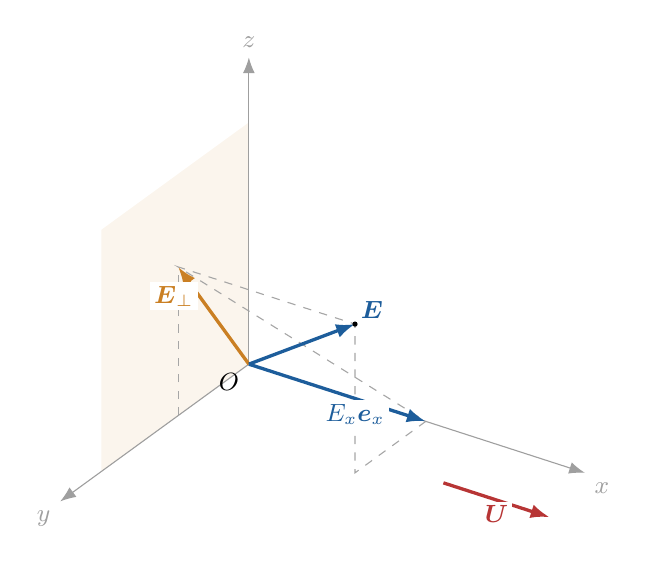
\begin{tikzpicture}[x={(.8320503cm,-.2690691cm)},y={(-.5547002cm,-.4036037cm)},z={(0cm,.8744746cm)},scale=1.35]
\coordinate (O) at (0,0,0);
\coordinate (A) at (2,0,0);
\coordinate (Y) at (0,1.2,0);
\coordinate (W) at (0,1.2,1.6);
\coordinate (V) at (2,1.2,1.6);
\fill[transverse!8] (O)--(0,2.5,0)--(0,2.5,2.6)--(0,0,2.6)--cycle;
\draw[proj] (A)--(2,1.2,0)--(V)--(W)--cycle;
\draw[proj] (Y)--(W);
\draw[axis] (O)--(3.8,0,0) node[below right] {$x$};
\draw[axis] (O)--(0,3.2,0) node[below left] {$y$};
\draw[axis] (O)--(0,0,3.3) node[above] {$z$};
\draw[vec,fieldblue] (O)--(A) node[pos=.6,below,lab] {$E_x\boldsymbol e_x$};
\draw[vec,transverse] (O)--(W) node[pos=.7,left,lab] {$\boldsymbol E_\perp$};
\draw[vec,fieldblue] (O)--(V) node[above right,lab] {$\boldsymbol E$};
\draw[vec,dipolered] (2.2,0,-.6)--(3.4,0,-.6) node[pos=.5,below,lab] {$\boldsymbol U$};
\node[below left] at (O) {$O$};
\fill (V) circle (.7pt);
\end{tikzpicture}

\begin{tikzpicture}[scale=1.1]
\foreach \shift/\label/\yp/\ang in {0/{S}/1/26.565051,5.3/{S'}/2/45}{
\begin{scope}[xshift=\shift cm]
\draw[axis] (0,0)--(3.55,0) node[right] {\ifdim \shift pt=0pt $x$\else $x'$\fi};
\draw[axis] (0,0)--(0,3.1) node[above] {$\boldsymbol e_\perp$};
\draw[proj] (2,0)--(2,\yp)--(0,\yp);
\draw[vec,fieldblue] (0,0)--(2,\yp);
\draw[fieldblue] (.7,0) arc[start angle=0,end angle=\ang,radius=.7];
\node[lab] at (1,-.35) {$E_x$};
\node[lab,left] at (0,\yp) {\ifdim \shift pt=0pt $E_\perp$\else $\gamma E_\perp$\fi};
\node at (1.65,3.3) {$\label$};
\ifdim \shift pt=0pt
\node[above right,lab] at (2,\yp) {$\boldsymbol E$};
\node[lab] at (.98,.23) {$\theta$};
\else
\node[above right,lab] at (2,\yp) {$\boldsymbol E'$};
\node[lab] at (.98,.33) {$\vartheta$};
\fi
\end{scope}
}
\node at (4.1,1.35) {$\gamma=2$};
\draw[-{Latex[length=2mm]},gray] (3.55,1.7)--(4.8,1.7);
\end{tikzpicture}

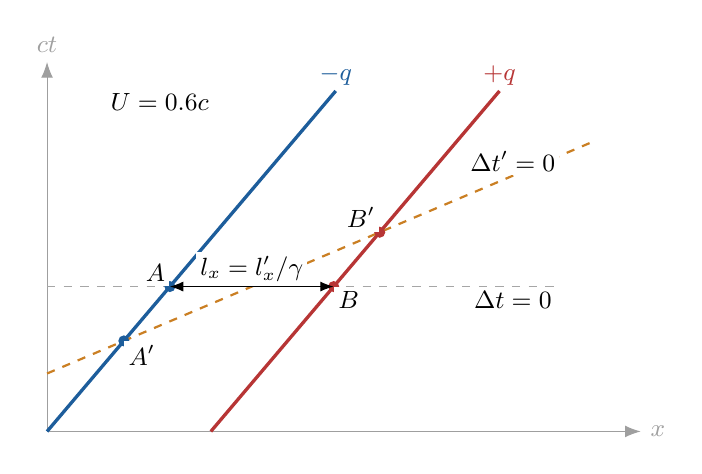
\begin{tikzpicture}[x=1.3cm,y=.92cm]
\draw[axis] (0,0)--(5.8,0) node[right] {$x$};
\draw[axis] (0,0)--(0,5.1) node[above] {$ct$};
\draw[very thick,fieldblue] (0,0)--(2.82,4.7) node[above,lab] {$-q$};
\draw[very thick,dipolered] (1.6,0)--(4.42,4.7) node[above,lab] {$+q$};
\draw[proj] (0,2)--(5.0,2);
\draw[transverse,dashed,thick] (0,.8)--(5.3,3.98);
\coordinate (A) at (1.2,2);
\coordinate (B) at (2.8,2);
\coordinate (Apr) at (.75,1.25);
\coordinate (Bpr) at (3.25,2.75);
\fill[fieldblue] (A) circle (2pt);
\fill[dipolered] (B) circle (2pt);
\fill[fieldblue] (Apr) circle (2pt);
\fill[dipolered] (Bpr) circle (2pt);
\node[lab,above left] at (A) {$A$};
\node[lab,below right] at (B) {$B$};
\node[lab,below right] at (Apr) {$A'$};
\node[lab,above left] at (Bpr) {$B'$};
\draw[{Latex[length=1.7mm]}-{Latex[length=1.7mm]},black] (A)--(B);
\node[lab,above] at (2,2) {$l_x=l'_x/\gamma$};
\node[lab,below] at (4.55,2) {$\Delta t=0$};
\node[lab,above] at (4.55,3.53) {$\Delta t'=0$};
\node[lab] at (1.1,4.55) {$U=0.6c$};
\end{tikzpicture}

\begin{tikzpicture}[scale=1.12]
\foreach \shift/\tag/\endx in {0/{S'}/2,5.8/{S}/1}{
\begin{scope}[xshift=\shift cm]
\draw[axis] (-.35,0)--(3.2,0) node[right] {\ifdim \shift pt=0pt $x'$\else $x$\fi};
\draw[axis] (0,-.35)--(0,2.9) node[above] {$\boldsymbol e_\perp$};
\draw[proj] (\endx,0)--(\endx,2)--(0,2);
\draw[vec,fieldblue] (0,0)--(\endx,2);
\filldraw[fill=white,draw=black] (0,0) circle (2.5pt);
\filldraw[fill=white,draw=black] (\endx,2) circle (2.5pt);
\node[lab,below left] at (0,0) {$-q$};
\node[lab,above right] at (\endx,2) {$+q$};
\node at (1.5,3.35) {$\tag$};
\ifdim \shift pt=0pt
\node[lab,above left] at (1,1) {$\boldsymbol l'$};
\node[lab,below] at (1,-.08) {$l'_x$};
\node[lab,left] at (-.05,1.95) {$l'_\perp$};
\else
\node[lab,above left] at (.5,1) {$\boldsymbol l$};
\node[lab,below] at (.5,-.08) {$l'_x/\gamma$};
\node[lab,left] at (-.05,1.95) {$l_\perp=l'_\perp$};
\fi
\end{scope}}
\node at (4.3,1.35) {$\gamma=2$};
\draw[-{Latex[length=2mm]},gray] (3.8,1.7)--(5.1,1.7);
\end{tikzpicture}

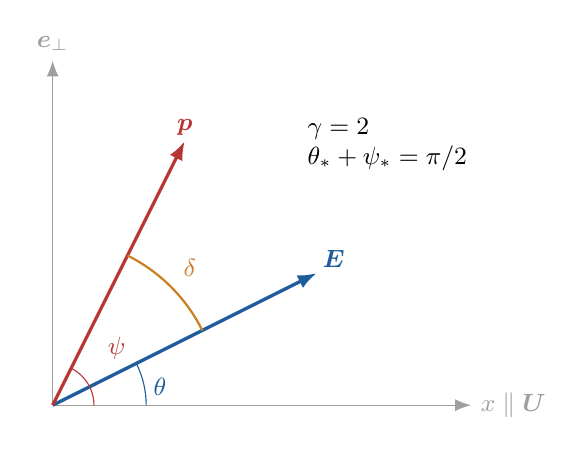
\begin{tikzpicture}[scale=1.25]
\draw[axis] (0,0)--(4.25,0) node[right] {$x\parallel\boldsymbol U$};
\draw[axis] (0,0)--(0,3.5) node[above] {$\boldsymbol e_\perp$};
\draw[vec,fieldblue] (0,0)--(2.683282,1.341641) node[above right,lab] {$\boldsymbol E$};
\draw[vec,dipolered] (0,0)--(1.341641,2.683282) node[above,lab] {$\boldsymbol p$};
\draw[fieldblue] (.95,0) arc[start angle=0,end angle=26.565051,radius=.95];
\node[fieldblue,lab] at (1.09,.19) {$\theta$};
\draw[dipolered] (.42,0) arc[start angle=0,end angle=63.434949,radius=.42];
\node[dipolered,lab] at (.65,.58) {$\psi$};
\draw[transverse,thick] (26.565051:1.7) arc[start angle=26.565051,end angle=63.434949,radius=1.7];
\node[transverse,lab] at (45:1.97) {$\delta$};
\node[align=left,lab] at (3.4,2.65) {$\gamma=2$\\$\theta_*+\psi_*=\pi/2$};
\end{tikzpicture}

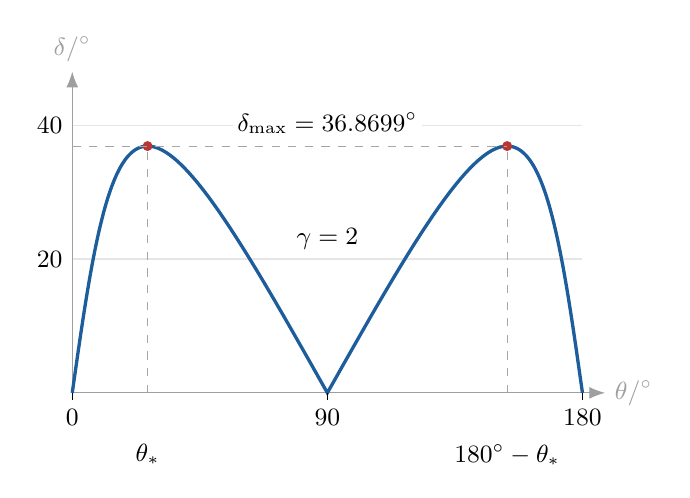
\begin{tikzpicture}[x=.036cm,y=.085cm]
\foreach \val in {20,40}{
\draw[gray!20] (0,\val)--(180,\val);
\node[left] at (0,\val) {$\val$};}
\draw[axis] (0,0)--(188,0) node[right] {$\theta/{}^\circ$};
\draw[axis] (0,0)--(0,48) node[above] {$\delta/{}^\circ$};
\draw[very thick,fieldblue] plot[domain=0:180,samples=361]
(\x,{atan(3*abs(sin(\x)*cos(\x))/(cos(\x)^2+4*sin(\x)^2))});
\foreach \xx in {26.565051,153.434949}{
\draw[proj] (\xx,0)--(\xx,36.869898);
\fill[dipolered] (\xx,36.869898) circle (1.8pt);}
\draw[proj] (0,36.869898)--(153.434949,36.869898);
\node[lab,above] at (90,38) {$\delta_{\max}=36.8699^\circ$};
\foreach \xx in {0,90,180}{\draw (\xx,0)--(\xx,-1); \node[below] at (\xx,-1) {$\xx$};}
\node[lab,below] at (26.565051,-7) {$\theta_*$};
\node[lab,below] at (153.434949,-7) {$180^\circ-\theta_*$};
\node[lab] at (90,23) {$\gamma=2$};
\end{tikzpicture}
\end{document}
